\documentclass[12pt]{article}
\usepackage[utf8]{inputenc}
\usepackage{amsmath, amsfonts, amssymb, amsthm, latexsym}
\usepackage{float}
\setlength{\parindent}{0in}
\setlength{\oddsidemargin}{0in}
\setlength{\textwidth}{6.5in}
\setlength{\textheight}{8.8in}
\setlength{\topmargin}{0in}
\setlength{\headheight}{18pt}

%%%%%%%%% IMAGES/FIGURES %%%%%%%%%

\usepackage{graphicx}
\usepackage{caption}
\DeclareCaptionFormat{citation}{%
  \ifx\captioncitation\relax\relax\else
    \captioncitation\par
  \fi
  #1#2#3\par}
\newcommand*\setcaptioncitation[1]{\def\captioncitation{\textit{Source:}~#1}}
\let\captioncitation\relax
\captionsetup{format=citation,justification=centering}

%%%%%%%%% LINKS %%%%%%%%%

\usepackage{hyperref}
\hypersetup{
    colorlinks=true,
    linkcolor=blue,
    filecolor=magenta,      
    urlcolor=cyan,
    pdftitle={Overleaf Example},
    pdfpagemode=FullScreen,
    }
\urlstyle{same}

\title{Random Math}
\author{Elijah Renner}

\begin{document}

\maketitle

\vspace{0.5in}

\tableofcontents

\section{Injectivity and Surjectivity}

\begin{figure}[H]
	\centering
	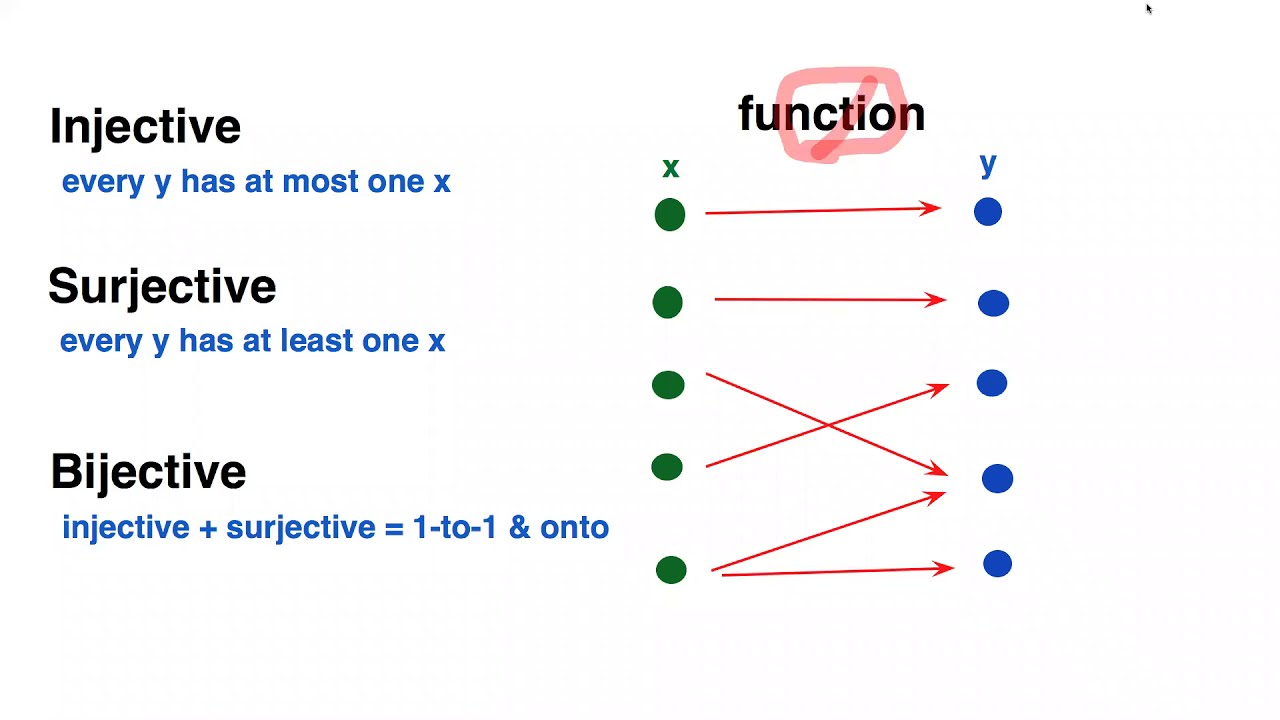
\includegraphics[scale=0.3]{media/maxresdefault.jpg}
\end{figure}

\section{Probability Notations}

The notation \(P(A)\) represents the probability that event \(A\) will occur.\\

\(P(A|B)\) represents the probability of \(A\) occuring given \(B\).\\

\(P(A')\) represents the probability of the complement of \(A\).
occuring.\\

\begin{figure}[H]
	\centering
	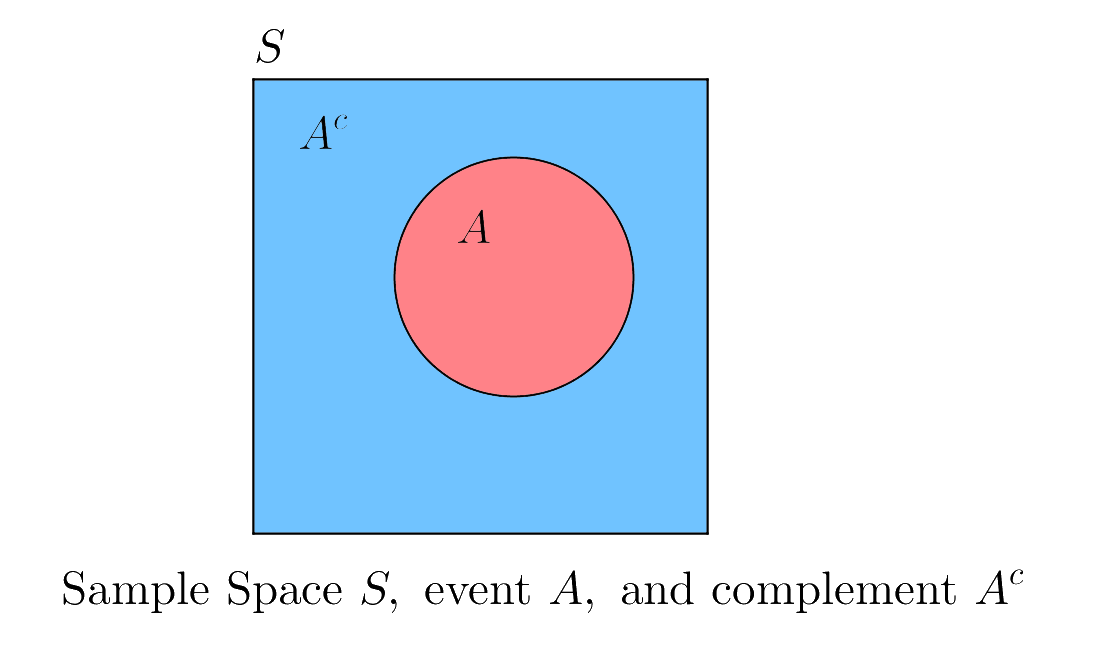
\includegraphics[scale=0.3]{media/compliment.png}
\end{figure}

\section{Binomial Coefficients}
 
In combinatorics, \textit{n} choose \textit{k}, denoted as \( \binom{n}{k} \), is the number of ways to choose \textit{k} elements from a set of \textit{n} distinct elements without regard to the order of selection. This concept is closely related to Pascal's Triangle and has applications in binomial expansions, probability theory, and other areas of mathematics.\\

The formula for \( n \choose k \) is given by:
\[
\binom{n}{k} = \frac{n!}{k!(n-k)!}
\]
where \( n! \) represents the factorial of \( n \) and is defined as the product of all positive integers from 1 to \( n \). This expression counts the number of ways to select \textit{k} elements from a set of \textit{n} elements.\\

For example, \( \binom{5}{2} \) is the number of ways to choose 2 elements from a set of 5, which is:
\[
\binom{5}{2} = \frac{5!}{2!(5-2)!} = \frac{5 \times 4}{2 \times 1} = 10
\]

\section{Pascal's Triangle}
Pascal's Triangle is a triangular array of binomial coefficients. Each entry in the triangle is equal to the sum of the two entries directly above it. The general structure of Pascal's Triangle is as follows:

\[
\begin{array}{cccccccc}
    &  &  & 1 &  &  &  &  \\
    &  & 1 &  & 1 &  &  &  \\
    & 1 &  & 2 &  & 1 &  &  \\
    1 &  & 3 &  & 3 &  & 1 &  \\
    \vdots & & \vdots &  & \vdots & & \vdots  \\
\end{array}
\]
Each entry \( \binom{n}{k} \) in Pascal's Triangle represents the number of ways to choose \textit{k} elements from a set of \textit{n} elements. The top row corresponds to \( n = 0 \), the next row to \( n = 1 \), and so on.

\section{Binomial Expansion}
The binomial theorem provides a formula for expanding expressions of the form \( (a + b)^n \). Using \( n \choose k \), the binomial expansion of \( (a + b)^n \) is given by:
\[
(a + b)^n = \sum_{k=0}^{n} \binom{n}{k} a^{n-k} b^k
\]
This formula expresses the powers of a binomial (i.e., \( a + b \)) as a sum of terms involving binomial coefficients. For example, expanding \( (a + b)^3 \) using the binomial theorem gives:
\[
(a + b)^3 = \binom{3}{0} a^3 b^0 + \binom{3}{1} a^2 b^1 + \binom{3}{2} a^1 b^2 + \binom{3}{3} a^0 b^3
\]
Simplifying the terms:
\[
(a + b)^3 = 1 \cdot a^3 + 3 \cdot a^2b + 3 \cdot ab^2 + 1 \cdot b^3 = a^3 + 3a^2b + 3ab^2 + b^3
\]
This result matches what we would expect from multiplying out the terms directly.


\end{document}
